\documentclass{article}
\usepackage[utf8]{inputenc}
\usepackage[T1]{fontenc}
\usepackage{graphicx}	% images PNG
\usepackage{geometry}	% margins
\usepackage{url}		% links
\usepackage{charter}	% betterfont
\usepackage{stmaryrd}	% math symbols ?
\usepackage{eso-pic}
\usepackage{siunitx}	% SI units
\usepackage{amsmath}	% advanced math symbols
\usepackage{rotating}
\usepackage{multirow}	
\usepackage{color, colortbl}	% color fonts and table backgrounds
\usepackage{titlesec}
\usepackage{enumitem}
\usepackage{notoccite}
\usepackage{fancyhdr}	% page headers/footers
\newcommand\BackgroundPic{\put(0,0){\parbox[b][\paperheight]{\paperwidth}{
\vfill
\centering

\includegraphics[width=\paperwidth,height=\paperheight,keepaspectratio]{background.png}
\vfill
}}}
\geometry{top=1.5cm,bottom=1.5cm, left=2cm, right=2cm}
\titlespacing*{\paragraph}{0pt}{0pt plus 0pt minus 0pt}{0pt plus 0pt minus 0pt}
\titlespacing*{\subsection}{0pt}{0pt plus 0pt minus 0pt}{0pt plus 0pt minus 0pt}
\titlespacing*{\itemize}{0pt}{0pt plus 0pt minus 0pt}{0pt plus 0pt minus 0pt}

\title{Intermediate Work Report:}
\author{Louis Becquey}
\date{\today}

\setlength\parskip{\baselineskip}

\pagestyle{fancy}
\setlength{\headheight}{14.7pt}
\fancyhead[L]{\textsc{IP framework inserting RNA motives}}
% \fancyhead[L]{\leftmark}
\fancyhead[R]{Louis Becquey}
\fancyfoot[L]{}
\fancyfoot[C]{}
\fancyfoot[R]{\thepage}
\begin{document}

\begin{titlepage}
	\AddToShipoutPicture*{\BackgroundPic}
	\begin{center}
		\vspace{3cm}
		\LARGE
		\textsc{Intermediate Work Report:}\\
		{\Large Louis Becquey, \today}\\
		\vspace{2cm}
		\textit{A biobjective IP framework that uses detected possible RNA modules\\ to predict RNA secondary structures}\\
	\end{center}
	\normalsize
	\vspace{5cm}
	
	\hrulefill
	\flushright{
		\textbf{under the supervision of:\\}
		Fariza Tahi, HDR \\
		Eric Angel, HDR \\
		\textit{AROBAS, IBISC, Paris-Saclay University}\\
		~ \\
		
\includegraphics[height=1cm]{logoIBISC.png} ~ ~ 
		
\includegraphics[height=1cm]{minisaclay.png}
	}
	\flushleft
	\hrulefill
\end{titlepage}

\section*{Graphical Abstract}
\begin{figure}[h]
	\hspace{-1.8cm}
	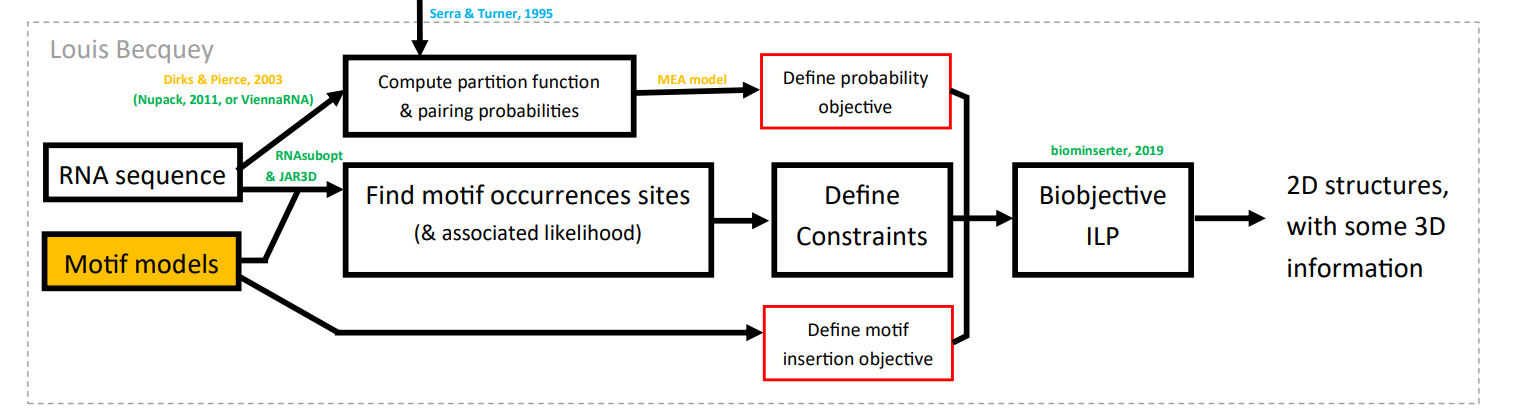
\includegraphics[width=1.2\linewidth]{graph_abstract.png}
\end{figure}
\tableofcontents

\newpage

\section{Motivation}
We now have quite consistent RNA module databases (RNA3Dmodule \cite{djelloul_automated_2008}, the RNA Motif Atlas \cite{petrov_automated_2013}, or CaRNAval \cite{reinharz2018mining}). 
We call a RNA module the combined description of these points:
\begin{itemize}
\item A particular base-pairing pattern of canonical \& wobble pairing (bi-dimensional information),
	\item A particular organisation of non-canonical contacts in space (tri-dimensional information).
	\item A sequence or consensus sequence that we know to adopt that particular base-pairing organisation (sequence information), or at least a probabilistic model to predict if a given sequence will fold according to the module.
\end{itemize}
Then, a RNA module is direct data about how a sequence can fold in space. Here, we are interested in using them to predict the bi or tri dimensional structure of an RNA sequence from scratch. 
Then, the algorithm we plan to use is the following:

\begin{itemize}
	\item Find all possible occurences of known RNA modules in the query sequence by using the sequence probabilistic models of the modules against the query bases,
	\item Define constraints on the secondary structure imposed by motives if they would be included
	\item Find a secondary structure that satisfies as much as possible both the expected accuracy of the structure and a criterion of module inclusion, by solving a bi-objective IP problem, using the previous constraints.
\end{itemize}

\section{Computation of basepair probabilities}
To compute the probability of a structure to exist in the equilibrium thermodynamical ensemble, we need to estimate the basepair probabilities.
This is usually done by a dynamic programming algorithm using an energy parameter model for base stackings in stems and energies of loops.
As we are supposed to allow the existence of pseudoknots, we chose the Dirks \& Pierce algorithm \cite{dirksAlgorithmComputingNucleic2004} and its C++ implementation called Nupack.

\paragraph{Discussion of that choice} ~ \\
The Dirks and Pierce algorithm has a complexity of \(O(N^5)\) instead of the usual \(O(N^3)\) algorithm, and its implementation in libNupack is even not parallel.
We may want to use a faster one (like ViennaRNA's one), even if it does not officialy supports pseudoknots.
Actually, to form a simple class of pseudoknots, an RNA needs to have a high likelihood to form each of the two independant loops in a non-pseudoknotted form. 
Then, using a probability matrix computed with an algorithm that does not model pseudoknot may result in similar structures. 
Our biobjective program would etablish the pseudoknot after all as forming more stems stabilizes the structure and as we do not forbid the pseudoknot.

\section{Detection of potential modules in the sequence input}
\paragraph{\textbf{Choice of a module model, choice of a sequence probabilistic model}} ~ \\
Depending on the authors and databases, different approaches have been published. 
A very complete model has been developped by the BGSU team \cite{zirbel_identifying_2015} : For each recurrent module of their "3D Motif Atlas", they build a probabilistic model for sequence variability based on a hybrid Stochastic Context-Free Grammar/Markov Random Field (SCFG/MRF) method.
Concerning the other databases, a probabilistic model using a bayesian Network can be designed for an RNA module \cite{cruz2011sequence} to estimate the probability that the sequence would fold into the module. 

As BGSU's model is already implemented in a software called JAR3D that perfectly suits our need, we decided to use BGSU's model of modules and their database.
JAR3D finds, given the sequence of an RNA loop with no additional information, the likelihood that it folds in every known 3D module of the RNA Motif Atlas \cite{petrov_automated_2013}.

For each module group of the database, JAR3D estimates the probability that a sequence folds into the 3D pattern, given instances of the module in real RNA 3D structures. 
The instances might differ in sequence, length of bulged insertions, and other details, but share a common graph of 3D non-canonical interactions.
It takes into account crossed contacts, base-ribose and base-phosphate interactions, and triple base-pairs.
This is the most complete approach to use to my knowledge.

\paragraph{\textbf{Detection of the loops in an RNA sequence}} ~ \\
As JAR3D scores the sequence of RNA loops, we first need to predict the 2D loops positions in the RNA sequence.

For now, we have been using RNAsubopt from the ViennaRNA package \cite{lorenz_viennarna_2011} to compute the 10 most probable 2D structures of the RNA and extract the loops that occur in those structures.
This computation should be avoided in the future : It requires the computation of the RNA's partition function and basepair probabilities again, which is something we already computed with Nupack.
Unfortunately, to avoid computing it twice, we should reimplement ourselves the algorithms instead of using the actual implementations. We have programs that output the basepair matrix but no structures, and programs that output structures but not the basepair matrix, and we don't have a program that can do both.

\section{Formulation of the IP problem}

This formulation is an improved merge between the IPknot \cite{sato_ipknot:_2011} formulation to fold RNAs with pseudoknots (but without "levels") and RNAMoIP's one \cite{reinharz_towards_2012} to include modules.
The bi-objective algorithm is inspired from BiokoP \cite{legendre_bi-objective_2018} and detailed later in section \ref{methods}.
% This problem has been inspired by IPknot's model \cite{sato_ipknot:_2011}, but without the use of what they call \textit{levels}, which are pseudoknot-free
% structures that should be superposed to give the true pseudoknotted secondary structure graph.\\
% Levels are mutually exclusive (a base cannot be paired in two different levels). The more levels you use, the more decision variables you have, 
% but the more complex pseudoknots you are able to predict. IPknot and BiokoP use 2 levels, to predict simple knots.\\
% \begin{figure}[h]\centering 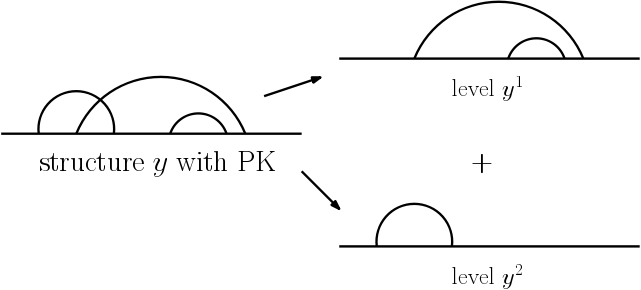
\includegraphics[height=5cm]{levels.png}\end{figure}


\subsection{Variables}

% Let $m$ be the number of levels that our program uses.\\
Let $n$ be the number of nucleotides in the query RNA sequence $s$.\\
Let $M$ be the set of modules that could be inserted in $s$ (a loop from $s$ has a good JAR3D score against one of the modules).\\
Let $x$ be a module of $M$, $\|x\|$ be the number of distinct components of $x$, and $p(x)$ the associated score of insertion given by JAR3D for that motif inserted at a particular position.\\
Let $P_{x,i}$ be the position in $s$ where we can insert the $i$th component of module $x$.\\
As the same module model can be inserted several times in $s$, several different $x$ modules in $M$ may refer to the same theoretical module, but inserted at different positions.\\
Let $k_{x,i}$ be the size in nucleotides of that $i$th component of $x$.\\
Let $y^u_v$ be the \textbf{decision boolean variable} indicating that $s[u]$ and $s[v]$ form a canonical base pairing. According to the standard loop model, we always have $v > u + 3$.\\
Let $C^x_i$ be the \textbf{decision boolean variable} indicating that we do insert the $i$th component of module $x$ at position $P_{x,i}$.


Note that a base pair $y^u_v$ is possible if and only if $v>u+3$, and that we do not need to use two variables $y^u_v$ and $y_{vu}$ for the same pair. 
Then, we have $\sum_{i=4}^n (n-i)$ decision variables ($\approx \frac{1}{2}n^2$ decision variables) of the form $y^u_v$.
Regarding the $C^x_i$, if we have an average insertion of $\nu$ motives by RNA sequence, the motives having in average $\mu$ components, components that can be inserted in average at $\pi$ different positions in $s$,
then we need to add, in average, $\nu \times \mu \times \pi$ decision variables $C^x_i$.

Then, we expect having around $\frac{1}{2}n^2+\nu \mu \pi$ decision variables.

\newpage
\subsection{Objectives \label{objectives}}
We have two objectives : Find a structure with correct expected accuracy, and find a structure which includes (large) known modules.
Let $X$ be the vector of all our decision variables, we define the following objective functions to maximize:
\[ f_{1A}(X) = \sum_{x \in M} (\|x\|)^2 \times C^x_1  \]
\[ f_{1B}(X) = \sum_{x \in M} p(x) \times C^x_1 \]
\[ f_{1C}(X) = \sum_{x \in M} \left[ \frac{\|x\|}{\log_2(\sum_{i=1}^{\|x\|}k_{x,i})} \times p(x) \times C^x_1 \right]\]
$$ f_2(X) = \sum_{u<v} p_{uv}\times y^u_v \times I[p_{uv}>\theta], \qquad \qquad
	p_{uv} = \sum_{\sigma \in S(s)} y^u_v.p(\sigma | s)$$
The different $f_1$ objectives are supposed to maximize the number of inserted motives in $s$, 
weighted by their number of components (squared for 1A), or the JAR3D score (B and C). 
In $1C$, a penalty is added on the number of nucleotides involved in the looped zone (sum of $k_{x,i}$) to avoid long unpaired zones. 
We don't know yet which one will give the better results.
$f_2$ is supposed to maximise the expected accuracy of the secondary structure. 
$p_{uv}$ are the base pairing probabilities.

Note that \(f_{1A}\) is taken from RNA MoIP \cite{reinharz_towards_2012}, to compare performance.

\subsection{9 Constraints to bind them all}
\paragraph{Constraint to ensure there only is 0 or 1 canonical pairing by nucleotide} ~ 
\begin{equation} \label{constraint:1}
	\sum_{v<u} y^v_u + \sum_{v>u} y^u_v \leq 1 \qquad\qquad \forall u \in \llbracket 1,n \rrbracket
\end{equation}

\paragraph{Constraints to forbid lonely base pairs} ~
% \begin{equation} \label{constraint:2}
% 	\sum_{v=u}^n y^{u-1}_v - \sum_{v=u+1}^n y^u_v + \sum_{v=u+2}^n y^{u+1}_v \geq 0 \qquad \qquad \forall u \in \llbracket 1,n\rrbracket
% \end{equation}
% \begin{equation} \label{constraint:3}
% 	\sum_{u=1}^{v-2} y^u_{v-1} - \sum_{u=1}^{v-1} y^u_v + \sum_{u=1}^{v} y^u_{v+1} \geq 0 \qquad \qquad \forall v \in \llbracket 1,n\rrbracket
% \end{equation}
% These conditions ensure that if a base pair exists with $s[i]$, 
% one of the adjacent bases is paired too. 
% Equation \ref{constraint:2} is useful if $s[u]$ is paired with $s[v>u]$ (a nucleotide later in the sequence), 
% and equation \ref{constraint:3} if $s[v]$ is paired with $s[u<v]$ (a nucleotide earlier in the sequence).
\begin{equation} \label{constraint:2}
	y^{u-1}_{v+1} - y^u_v + y^{u+1}_{v-1} \geq 0 \qquad \qquad \forall (u,v) \in \{ (u,v) \in \llbracket 1,n\rrbracket^2 \; | \; u + 3 <v \}
\end{equation}
A basepair should be accompanied by one of its neighbours, forming a stable structure stabilized by stacking energies. In theory, this might add up to \( \frac{1}{2}n^2\) constraints, but in practice, this number is very reasonable as
the only decision variables kept are those with probability above a $\theta$ threshold. 
Then, this condition sets to zero "lonely decision variables" who have no neighbour basepair variable allowed.


\paragraph{Constraint to forbid pairings inside a module component} ~ 
\begin{equation} \label{constraint:4}
	(k_{x,i}-2) \; C^x_i + \sum_{u=P_{x,i}+1}^{P_{x,i}+k_{x,i}-2}\left[ \sum_{v>u} y^u_v + \sum_{v<u} y^v_u \right] \leq (k_{x,i} - 2)
	\qquad \qquad \forall x \in M, i \in \llbracket 1,\|x\| \rrbracket
\end{equation}

\paragraph{Constraint to forbid component to overlap} ~
\begin{equation} \label{constraint:5}
	\sum_{x \in M} \sum_{i=1}^{\|x\|} C^x_i \times I( u \in [ P_{x,i} ; P_{x,i}+k_{x,i}-1]) \leq 1 \qquad \qquad \forall u \in \llbracket 1,n \rrbracket
\end{equation}
$I( u \in [ P_{x,i} ; P_{x,i}+k_{x,i}-1])$ is a booleean value depending on the condition's truth. Then, whatever the nucleotide $u$, it can be part of a module component only once.
% \begin{center}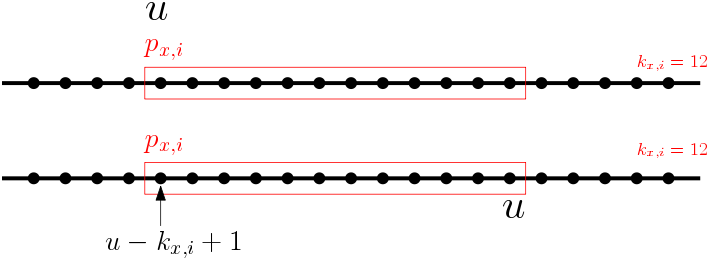
\includegraphics[height=3cm]{component.png}\end{center}

\paragraph{Constraints to respect the structure of large motives ($\{ x\in M \; | \; \|x\| \geq 2\}$)} ~ 

This constraint ensures that none or all the components of a motif are inserted.
\begin{equation}\label{constraint:6}
	\sum_{i=2}^{\|x\|} C^x_i = (\|x\| - 1) \times C^{x}_{1}	 \qquad \qquad \forall x \in \{ x\in M \; | \; \|x\| \geq 2\}
\end{equation}

And then, we force base pairs between the end of a component and the beginning of the next one:
\begin{equation}\label{constraint:7}
	C^x_1 \leq y^{P_{x,1}}_{P_{x,\|x\|}+k_{x,\|x\|}-1} \qquad \qquad \forall x \in \{ x\in M \; | \; \|x\| \geq 2\}
\end{equation}
\begin{equation}\label{constraint:8}
	C^x_j \leq y^{P_{x,j}+k_{x,j}-1}_{P_{x,j+1}} \qquad \qquad \forall x \in \{ x\in M \; | \; \|x\| \geq 2\}, \forall j \in \llbracket 1,\|x\| \llbracket
\end{equation}

Constraint \ref{constraint:7} binds the first nucleotide of first component to the last one of the last component. 
Constraint \ref{constraint:8} binds the last nucleotide of component $j$ to the first of component $j+1$.

\paragraph{Constraint to forbid a previously found solution} ~ 

As several solutions may result in the same values of the two objectives, we can't forbid the algorithm to search twice the same region of the objective landscape.
We have to explicitly forbid to find again every found solution.\\
We do it by adding iteratively, for every structure $s^*$ found, the following condition :
\begin{equation}\label{constraint:9}
	\sum_{y^u_v \in \{ y^u_v  | y^u_v = 1 \text{ in } s^* \}} (1 - y^u_v) + \sum_{y^u_v \in \{ y^u_v  | y^u_v = 0 \text{ in } s^* \}} y^u_v +
	\sum_{C^x_i \in \{ C^x_i  | C^x_i = 1 \text{ in } s^* \}} (1 - C^x_i) + \sum_{C^x_i \in \{ C^x_i  |C^x_i = 0 \text{ in } s^* \}} C^x_i \geq 1
\end{equation}

It ensures that at least one of the decision variables differs from $s^*$.

\section{Methods \label{methods}}
\subsection{Bi-objective algorithm}
This is an adaptation of BiokoP's algorithm \cite{legendre_bi-objective_2018} to gather all the points of the pareto set, removing the $k$-pareto set part.

We start by solving each objective independantly to have a lower and higher bound on each objective. 
The two solutions found are considered optimal (higher bound) on one objective, and the worse point of the Pareto set concerning the other objective.

Then, we will iteratively solve the mono-objective problem, but adding as a constraint that the second one has to be included between the bounds.
Suppose we decide to iteratively solve objective 1. 
The found solutions are getting worse and worse concerning objective 1, but better and better concerning objective 2. 
Every time a solution is found with a better objective 2 value, we update our lower bound to search for solutions with objective 2 above this new value.
Note that we use weak inequality constraints, as several solutions may have the same values concerning the two objectives and that we want to include them in the Pareto set.

When no more solutions are discovered, the Pareto has been entirely found.

\subsection{Solving the IP problem}
We use ILOG CPLEX's \cite{cplex} concert technology to solve the integer linear programming problem. All our decision variables are booleans, and all our constraints are linear.

\subsection{Benchmarking of the module inclusion objective functions}
To assess the performance of the objective functions proposed in section \ref{objectives}, we need to chose some performance metrics.
We will focus on:
\begin{itemize}
	\item wether the native secondary structure of the proposed RNA sequence exists in the returned solutions (the pareto set),
	\item the number of solutions returned (size of the Pareto set).
\end{itemize}

The performance is assessed on the structures taken from the RNA STRAND database \cite{andronescu2008rna}, after a simple preprocessing to remove pseudobases.

\section{Results \label{results}}
\subsection{Comparison of the 3 objective functions for motif insertion}
It appears that function $f_{1A}$ introduced in section \ref{objectives} is not usable in practice.
Actually, on a short RNA sequence (67 nucleotides) but with 4 loop sites that may fold into $~30$ different known loops, 
we obtain a combinatorial superposition of near $30^4 = 810 000$ structures which have the same $f_{1A}$ and $f_2$ objectives values, and 
all belong to the Pareto front. This results is not desired, as the size of the Pareto set is wanted to be small, and as the program fills the machine's memory very quick in practice.

\section{Discussion \label{discussion}}


%%%%%%%%%%%%%%%%%%%%%%%%%%%%%%%%%%%%%%%%%%%%%%%%%%%%%%%%%%%%%%%%%%%%%%%%%%%%%%%%%%%%%%%%%%%%%%%%%%%%%%
% \newpage
\bibliographystyle{unsrt}
\bibliography{RNA}
\end{document}